% This file was created with tikzplotlib v0.10.1.
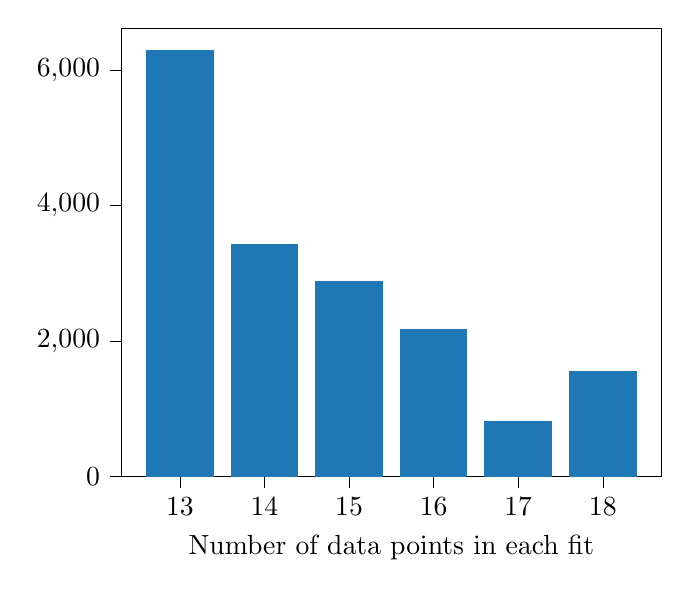
\begin{tikzpicture}

\definecolor{darkgray176}{RGB}{176,176,176}
\definecolor{steelblue31119180}{RGB}{31,119,180}

\begin{axis}[
tick align=outside,
tick pos=left,
x grid style={darkgray176},
xlabel={Number of data points in each fit},
xmin=12.31, xmax=18.69,
xtick style={color=black},
y grid style={darkgray176},
ymin=0, ymax=6622.35,
ytick style={color=black}
]
\draw[draw=none,fill=steelblue31119180] (axis cs:12.6,0) rectangle (axis cs:13.4,6307);
\draw[draw=none,fill=steelblue31119180] (axis cs:13.6,0) rectangle (axis cs:14.4,3441);
\draw[draw=none,fill=steelblue31119180] (axis cs:14.6,0) rectangle (axis cs:15.4,2886);
\draw[draw=none,fill=steelblue31119180] (axis cs:15.6,0) rectangle (axis cs:16.4,2177);
\draw[draw=none,fill=steelblue31119180] (axis cs:16.6,0) rectangle (axis cs:17.4,816);
\draw[draw=none,fill=steelblue31119180] (axis cs:17.6,0) rectangle (axis cs:18.4,1559);
\end{axis}

\end{tikzpicture}
